% !TEX root = ../../seminar.tex

\section{Research Process - \checklist}
\label{sec:research process}

\begin{minipage}{\linewidth}
\begin{wrapfigure}{R}{0.3\textwidth}
	\centering
	\vspace{1cm}
	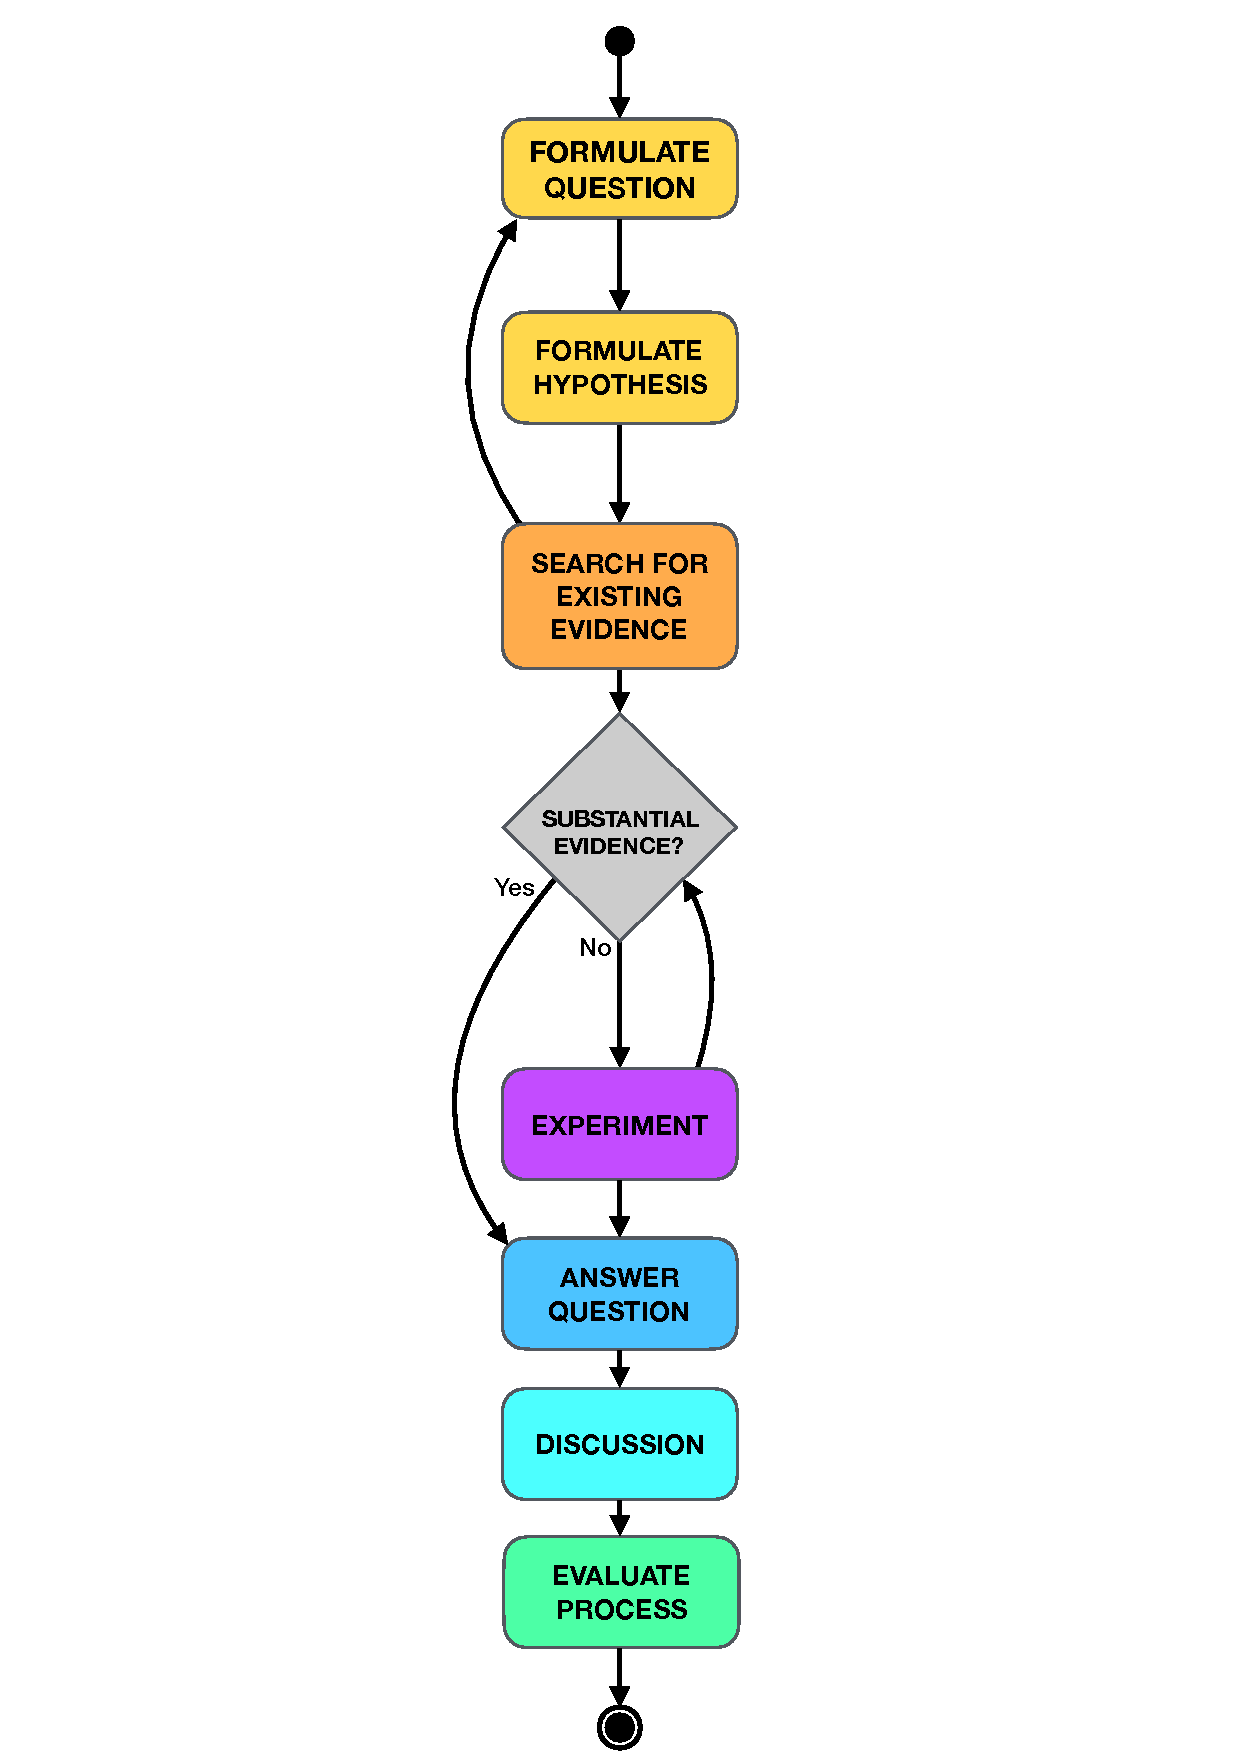
\includegraphics[trim={3cm 0 3cm 0}, height=17cm]{figures/workflow_graph.pdf}
	\caption{Workflow Graph}
	\label{fig:workflow_graph}
\end{wrapfigure}



\todo{Motivation}\\
Rainer \etal found, that \q{[s]tudents varied in their use of the EBSE checklist}\cite{Rainer2006} (see issue \ref{itm:issue5} in table \ref{table:issuesEBSE}). Therefore, \checklist is designed to support students during the process and with doing \todosoft{rephrase} EBSE rather than cluttering the process even more.

The process of \checklist \todosoft{rephrase} contains seven steps and one branch point: "Formulate question", "formulate hypothesis", "search for existing evidence", "experiment", "answer question", "discussion", "evaluate process", and "substantial evidence?".

In the left column of the document is a flow chart of the proposed process depicted. For computer science students this should be a fast way to navigate through the process. To further assist navigation visually each process step has been assigned a color to.

In the right column additional information is given about the process steps. Each process step in \checklist contains a short description, some guidelines, and a checklist with acceptance criteria. Whereas the guidelines contain methods and tool on how to process the current step. And the acceptance criteria give students a hint on when the current step is completed and move on to the next step in the process.

\subsection{Test}
\lipsum[1]

\end{minipage}

